\documentclass{standalone}
\usepackage{tikz}
\usetikzlibrary{patterns, positioning}


\begin{document}
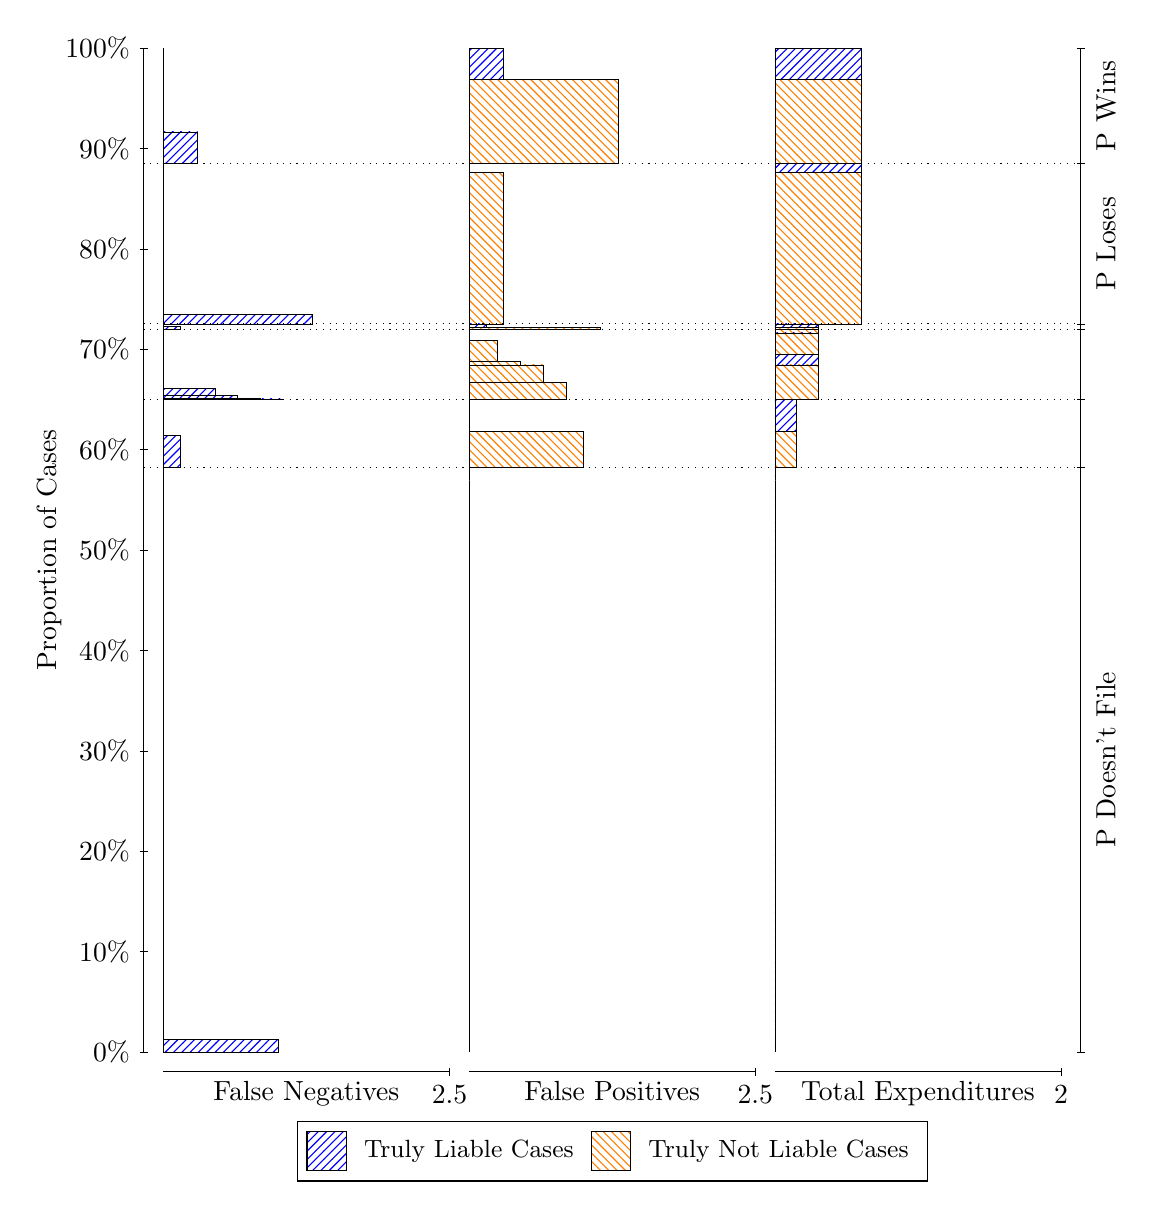
\begin{tikzpicture}
\draw[black, very thin] (1.5,1.75) -- (1.5,14.5);
\node[rotate=90, text=black, anchor=center] at (0.3, 8.125) {Proportion of Cases};
\draw[black, very thin] (1.45,1.75) -- (1.55,1.75);
\node[text=black, anchor=east] at (1.45, 1.75) {0\%};
\draw[black, very thin] (1.45,3.025) -- (1.55,3.025);
\node[text=black, anchor=east] at (1.45, 3.025) {10\%};
\draw[black, very thin] (1.45,4.3) -- (1.55,4.3);
\node[text=black, anchor=east] at (1.45, 4.3) {20\%};
\draw[black, very thin] (1.45,5.575) -- (1.55,5.575);
\node[text=black, anchor=east] at (1.45, 5.575) {30\%};
\draw[black, very thin] (1.45,6.85) -- (1.55,6.85);
\node[text=black, anchor=east] at (1.45, 6.85) {40\%};
\draw[black, very thin] (1.45,8.125) -- (1.55,8.125);
\node[text=black, anchor=east] at (1.45, 8.125) {50\%};
\draw[black, very thin] (1.45,9.4) -- (1.55,9.4);
\node[text=black, anchor=east] at (1.45, 9.4) {60\%};
\draw[black, very thin] (1.45,10.675) -- (1.55,10.675);
\node[text=black, anchor=east] at (1.45, 10.675) {70\%};
\draw[black, very thin] (1.45,11.95) -- (1.55,11.95);
\node[text=black, anchor=east] at (1.45, 11.95) {80\%};
\draw[black, very thin] (1.45,13.225) -- (1.55,13.225);
\node[text=black, anchor=east] at (1.45, 13.225) {90\%};
\draw[black, very thin] (1.45,14.5) -- (1.55,14.5);
\node[text=black, anchor=east] at (1.45, 14.5) {100\%};

\draw[black, very thin] (13.4,1.75) -- (13.4,14.5);
\draw[black, very thin] (13.35,1.75) -- (13.45,1.75);
\node[anchor=west] at (13.35, 1.75) {};
\draw[black, very thin] (13.35,9.1706) -- (13.45,9.1706);
\node[anchor=west] at (13.35, 9.1706) {};
\draw[black, very thin] (13.35,10.037) -- (13.45,10.037);
\node[anchor=west] at (13.35, 10.037) {};
\draw[black, very thin] (13.35,10.927) -- (13.45,10.927);
\node[anchor=west] at (13.35, 10.927) {};
\draw[black, very thin] (13.35,10.997) -- (13.45,10.997);
\node[anchor=west] at (13.35, 10.997) {};
\draw[black, very thin] (13.35,13.035) -- (13.45,13.035);
\node[anchor=west] at (13.35, 13.035) {};
\draw[black, very thin] (13.35,14.5) -- (13.45,14.5);
\node[anchor=west] at (13.35, 14.5) {};

\draw[black, very thin, pattern color=blue, pattern=north east lines] (1.75,1.75) rectangle (3.2033,1.9144);
\draw[black, very thin, pattern color=orange, pattern=north west lines] (1.75,1.9144) rectangle (1.75,9.1706);
\draw[black, very thin, pattern color=blue, pattern=north east lines] (1.75,9.1706) rectangle (1.968,9.5785);
\draw[black, very thin, pattern color=orange, pattern=north west lines] (1.75,9.5785) rectangle (1.75,10.037);
\draw[black, very thin, pattern color=blue, pattern=north east lines] (1.75,10.037) rectangle (3.276,10.043);
\draw[black, very thin, pattern color=blue, pattern=north east lines] (1.75,10.043) rectangle (2.9853,10.046);
\draw[black, very thin, pattern color=blue, pattern=north east lines] (1.75,10.046) rectangle (2.6947,10.085);
\draw[black, very thin, pattern color=blue, pattern=north east lines] (1.75,10.085) rectangle (2.404,10.18);
\draw[black, very thin, pattern color=orange, pattern=north west lines] (1.75,10.18) rectangle (1.75,10.927);
\draw[black, very thin, pattern color=blue, pattern=north east lines] (1.75,10.927) rectangle (1.968,10.969);
\draw[black, very thin, pattern color=orange, pattern=north west lines] (1.75,10.969) rectangle (1.75,10.997);
\draw[black, very thin, pattern color=blue, pattern=north east lines] (1.75,10.997) rectangle (3.6393,11.115);
\draw[black, very thin, pattern color=orange, pattern=north west lines] (1.75,11.115) rectangle (1.75,13.035);
\draw[black, very thin, pattern color=blue, pattern=north east lines] (1.75,13.035) rectangle (2.186,13.435);
\draw[black, very thin, pattern color=orange, pattern=north west lines] (1.75,13.435) rectangle (1.75,14.5);
\draw[black, very thin, pattern color=orange, pattern=north west lines] (5.6333,1.75) rectangle (5.6333,9.0062);
\draw[black, very thin, pattern color=blue, pattern=north east lines] (5.6333,9.0062) rectangle (5.6333,9.1706);
\draw[black, very thin, pattern color=orange, pattern=north west lines] (5.6333,9.1706) rectangle (7.0867,9.6292);
\draw[black, very thin, pattern color=blue, pattern=north east lines] (5.6333,9.6292) rectangle (5.6333,10.037);
\draw[black, very thin, pattern color=orange, pattern=north west lines] (5.6333,10.037) rectangle (6.8687,10.257);
\draw[black, very thin, pattern color=orange, pattern=north west lines] (5.6333,10.257) rectangle (6.578,10.476);
\draw[black, very thin, pattern color=orange, pattern=north west lines] (5.6333,10.476) rectangle (6.2873,10.518);
\draw[black, very thin, pattern color=orange, pattern=north west lines] (5.6333,10.518) rectangle (5.9967,10.783);
\draw[black, very thin, pattern color=blue, pattern=north east lines] (5.6333,10.783) rectangle (5.6333,10.927);
\draw[black, very thin, pattern color=orange, pattern=north west lines] (5.6333,10.927) rectangle (7.3047,10.955);
\draw[black, very thin, pattern color=blue, pattern=north east lines] (5.6333,10.955) rectangle (5.8513,10.997);
\draw[black, very thin, pattern color=orange, pattern=north west lines] (5.6333,10.997) rectangle (6.0693,12.918);
\draw[black, very thin, pattern color=blue, pattern=north east lines] (5.6333,12.918) rectangle (5.6333,13.035);
\draw[black, very thin, pattern color=orange, pattern=north west lines] (5.6333,13.035) rectangle (7.5227,14.1);
\draw[black, very thin, pattern color=blue, pattern=north east lines] (5.6333,14.1) rectangle (6.0693,14.5);
\draw[black, very thin, pattern color=orange, pattern=north west lines] (9.5167,1.75) rectangle (9.5167,9.0062);
\draw[black, very thin, pattern color=blue, pattern=north east lines] (9.5167,9.0062) rectangle (9.5167,9.1706);
\draw[black, very thin, pattern color=orange, pattern=north west lines] (9.5167,9.1706) rectangle (9.7892,9.6292);
\draw[black, very thin, pattern color=blue, pattern=north east lines] (9.5167,9.6292) rectangle (9.7892,10.037);
\draw[black, very thin, pattern color=orange, pattern=north west lines] (9.5167,10.037) rectangle (10.062,10.476);
\draw[black, very thin, pattern color=blue, pattern=north east lines] (9.5167,10.476) rectangle (10.062,10.61);
\draw[black, very thin, pattern color=orange, pattern=north west lines] (9.5167,10.61) rectangle (10.062,10.875);
\draw[black, very thin, pattern color=blue, pattern=north east lines] (9.5167,10.875) rectangle (10.062,10.881);
\draw[black, very thin, pattern color=orange, pattern=north west lines] (9.5167,10.881) rectangle (10.062,10.924);
\draw[black, very thin, pattern color=blue, pattern=north east lines] (9.5167,10.924) rectangle (10.062,10.927);
\draw[black, very thin, pattern color=orange, pattern=north west lines] (9.5167,10.927) rectangle (10.062,10.955);
\draw[black, very thin, pattern color=blue, pattern=north east lines] (9.5167,10.955) rectangle (10.062,10.997);
\draw[black, very thin, pattern color=orange, pattern=north west lines] (9.5167,10.997) rectangle (10.607,12.918);
\draw[black, very thin, pattern color=blue, pattern=north east lines] (9.5167,12.918) rectangle (10.607,13.035);
\draw[black, very thin, pattern color=orange, pattern=north west lines] (9.5167,13.035) rectangle (10.607,14.1);
\draw[black, very thin, pattern color=blue, pattern=north east lines] (9.5167,14.1) rectangle (10.607,14.5);
\draw[black, dotted] (1.5,9.1706) -- (13.4,9.1706);
\draw[black, dotted] (1.5,10.037) -- (13.4,10.037);
\draw[black, dotted] (1.5,10.927) -- (13.4,10.927);
\draw[black, dotted] (1.5,10.997) -- (13.4,10.997);
\draw[black, dotted] (1.5,13.035) -- (13.4,13.035);
\draw[black, very thin] (1.75,1.5) -- (5.3833,1.5);
\node[text=black, anchor=north] at (3.5667, 1.5) {False Negatives};
\draw[black, very thin] (5.3833,1.45) -- (5.3833,1.55);
\node[text=black, anchor=north] at (5.3833, 1.45) {2.5};

\draw[black, very thin] (5.6333,1.5) -- (9.2667,1.5);
\node[text=black, anchor=north] at (7.45, 1.5) {False Positives};
\draw[black, very thin] (9.2667,1.45) -- (9.2667,1.55);
\node[text=black, anchor=north] at (9.2667, 1.45) {2.5};

\draw[black, very thin] (9.5167,1.5) -- (13.15,1.5);
\node[text=black, anchor=north] at (11.333, 1.5) {Total Expenditures};
\draw[black, very thin] (13.15,1.45) -- (13.15,1.55);
\node[text=black, anchor=north] at (13.15, 1.45) {2};

\node[text=black, centered, rotate=90] at (13.72, 5.4603) {P Doesn't File};



\node[text=black, centered, rotate=90] at (13.72, 12.016) {P Loses};
\node[text=black, centered, rotate=90] at (13.72, 13.767) {P Wins};

\draw (7.449999999999999,1.5) node[draw=none] (baseCoordinate) {};
\begin{scope}[align=center]
        \matrix[scale=0.5, draw=black, below=0.5cm of baseCoordinate, nodes={draw}, column sep=0.1cm]{
            \node[rectangle, draw, minimum width=0.5cm, minimum height=0.5cm, pattern color=blue, pattern=north east lines] {}; &
            \node[draw=none, font=\small, text=black] (B) {Truly Liable Cases}; &
            \node[rectangle, draw, minimum width=0.5cm, minimum height=0.5cm, pattern color=orange, pattern=north west lines] {}; &
            \node[draw=none, font=\small, text=black] (B) {Truly Not Liable Cases}; \\
            };
\end{scope}

\end{tikzpicture}
\end{document}